% Options for packages loaded elsewhere
\PassOptionsToPackage{unicode}{hyperref}
\PassOptionsToPackage{hyphens}{url}
%
\documentclass[
]{scrartcl}
\usepackage{amsmath,amssymb}
\usepackage{lmodern}
\usepackage{iftex}
\ifPDFTeX
  \usepackage[T1]{fontenc}
  \usepackage[utf8]{inputenc}
  \usepackage{textcomp} % provide euro and other symbols
\else % if luatex or xetex
  \usepackage{unicode-math}
  \defaultfontfeatures{Scale=MatchLowercase}
  \defaultfontfeatures[\rmfamily]{Ligatures=TeX,Scale=1}
\fi
% Use upquote if available, for straight quotes in verbatim environments
\IfFileExists{upquote.sty}{\usepackage{upquote}}{}
\IfFileExists{microtype.sty}{% use microtype if available
  \usepackage[]{microtype}
  \UseMicrotypeSet[protrusion]{basicmath} % disable protrusion for tt fonts
}{}
\makeatletter
\@ifundefined{KOMAClassName}{% if non-KOMA class
  \IfFileExists{parskip.sty}{%
    \usepackage{parskip}
  }{% else
    \setlength{\parindent}{0pt}
    \setlength{\parskip}{6pt plus 2pt minus 1pt}}
}{% if KOMA class
  \KOMAoptions{parskip=half}}
\makeatother
\usepackage{xcolor}
\IfFileExists{xurl.sty}{\usepackage{xurl}}{} % add URL line breaks if available
\IfFileExists{bookmark.sty}{\usepackage{bookmark}}{\usepackage{hyperref}}
\hypersetup{
  pdftitle={Topological Aspects of Symmetry in Low Dimensions},
  pdfauthor={Kantaro Ohmori},
  hidelinks,
  pdfcreator={LaTeX via pandoc}}
\urlstyle{same} % disable monospaced font for URLs
\usepackage{longtable,booktabs,array}
\usepackage{calc} % for calculating minipage widths
% Correct order of tables after \paragraph or \subparagraph
\usepackage{etoolbox}
\makeatletter
\patchcmd\longtable{\par}{\if@noskipsec\mbox{}\fi\par}{}{}
\makeatother
% Allow footnotes in longtable head/foot
\IfFileExists{footnotehyper.sty}{\usepackage{footnotehyper}}{\usepackage{footnote}}
\makesavenoteenv{longtable}
\usepackage{graphicx}
\makeatletter
\def\maxwidth{\ifdim\Gin@nat@width>\linewidth\linewidth\else\Gin@nat@width\fi}
\def\maxheight{\ifdim\Gin@nat@height>\textheight\textheight\else\Gin@nat@height\fi}
\makeatother
% Scale images if necessary, so that they will not overflow the page
% margins by default, and it is still possible to overwrite the defaults
% using explicit options in \includegraphics[width, height, ...]{}
\setkeys{Gin}{width=\maxwidth,height=\maxheight,keepaspectratio}
% Set default figure placement to htbp
\makeatletter
\def\fps@figure{htbp}
\makeatother
\setlength{\emergencystretch}{3em} % prevent overfull lines
\providecommand{\tightlist}{%
  \setlength{\itemsep}{0pt}\setlength{\parskip}{0pt}}
\setcounter{secnumdepth}{5}
\usepackage{braket}
\ifLuaTeX
  \usepackage{selnolig}  % disable illegal ligatures
\fi
\usepackage[]{biblatex}
\addbibresource{ref.bib}

\title{Topological Aspects of Symmetry in Low Dimensions}
\author{Kantaro Ohmori}
\date{2022-02-07}

\begin{document}
\maketitle
\begin{abstract}
This is a lecture note prepared for ``26th APCTP Winter School on Fundamental Physics'', Feb.~14-18, 2022.

In this lecture we will study the symmetry and its anomaly in low-dimensional, i.e.~0+1d and 1+1d, quantum field theories.
In 0+1-dimensional quantum field theory, a.k.a quantum mechanics, the Wigner's theorem tells that a global symmetry forms a group and acts on the Hilbert (state) space as a projective representation. We will see example with non-trivial projective phases and how it can be related to symmetry protected topological phases in 1+1-dimensions. We then see how the story are generalized/changed in 1+1-dimensional (relativistic) quantum field theory, where the locality of the theory plays an important role.
Time permits, we also see how the inclusion of fermions affects the story.
\end{abstract}

{
\setcounter{tocdepth}{2}
\tableofcontents
}
\hypertarget{introduction}{%
\section{Introduction}\label{introduction}}

\[\ket{x}\]

\(\bra{x}, \braket{x|y|z}\)

Symmetry is a guiding principle in physics. In many case, given a system, you first analyze its symmetry. Or, to model a given phenomena, the symmetry is often be the first clue.
Therefore, there have been numerous research on the topic. What is surprising is that, still, in 2022, it is a hot area of research and there are many things to be understood.

\hypertarget{lecture-guide}{%
\subsection{Lecture Guide}\label{lecture-guide}}

\hypertarget{objective}{%
\subsubsection{Objective}\label{objective}}

This lecture aims to be an introduction to the field of symmetry and its anomaly in quantum field theory (QFT). In the first part of the lecture topological aspects of symmetry in quantum mechanics are reviewed, then in the latter part of the lecture we proceed to symmetry in 1+1-dimensional quantum field theory.

Proficiency in the undergraduate level quantum mechanics and some basic knowledge about quantum field theory are assumed, but (hopefully) not much more. Especially, the first half will focus on quantum mechanics so it is hopefully understandable to even advanced undergraduates.

\hypertarget{useful-references}{%
\subsubsection{Useful references}\label{useful-references}}

\begin{enumerate}
\def\labelenumi{\arabic{enumi}.}
\tightlist
\item
  \textcite{tachikawa_2019}:
  The first half of Yuji's lecture is about the big framework the most of researchers assume (but not necessarily proven), which I will omit.
  The second half of Yuji's will serve as an advanced version of this lecture.
\item
  \textcite{Witten:2015aoa}, \textcite{Witten:2015aba}:
  While there are not so much overlap between this lecture by me and these lecture note and paper by E. Witten, and Witten's is a bit more advanced, they are undoubtedly ones of the best entry points to the field.
\end{enumerate}

\hypertarget{motivation}{%
\subsection{Motivation}\label{motivation}}

Why do we care about symmetry and its anomaly in quantum field theory?
There are two (closely related) uses cases of symmetry and its anomaly in the study of QFT and its applications:

\begin{enumerate}
\def\labelenumi{\arabic{enumi}.}
\tightlist
\item
  to construction of a model, given observed spectrum or other desired properties, and
\item
  to constraining possible long range physics from 't Hooft anomaly matching.
\end{enumerate}

An example for the case one is the Standard Model (SM) of the particle physics.
The spectrum of the fermions fits into a representation of \(SU(3)\times SU(2) \times U(1)\) nicely, and gauging of the symmetry, after including the Higgs boson, magically explains almost all physics that occur in a collider. (The finding of the quark model involving the color symmetry was also mainly from group theory: it was to reproduce the observed \(SU(3)\) symmetry among hadrons. )

The quantum anomaly is also very important in construction of the SM: a single family of fermions in SM has chiral spectrum but seemingly miraculous cancellation of the quantum anomaly, which makes the model consistent. This cancellation also leads to the idea of grand unification.

The second case is about the quantum anomaly for \emph{global} symmetry.\footnote{Some authors, including the author of this lecture note, sometimes use the term ``'t Hooft anomaly'', to mean a quantum anomaly for a \emph{global} symmetry, to distinguish it from a quantum anomaly involving \emph{gauge} symmetry. However this terminology does not seem to have a historical root (while the term ``'t Hooft anomaly matching'' is easily justified), so in this lecture KO tries to avoid the terminology to avoid any possible confusion.}
't Hooft anomaly matching states that the anomaly should match between the UV and IR of an renormalization group (RG) flow (see Fig. \ref{fig:flow}).
Let \(G_\text{UV}\) and \(G_\text{IR}\) be the symmetry group for the UV and IR theory, respectively.
The existence of the RG flow between them in particular means that an isomorphism between them:
\begin{equation}
  \label{eq:Ghom}
  \phi: G_\text{UV} \to G_\text{IR}.
\end{equation}
The RG flow also assigns a map between the quantum anomalies, which are a property of symmetries in a local quantum system, for the symmetries \(G_\text{UV}\) and \(G_\text{IR}\);
but this time it is backwards:
\begin{equation}
  \label{eq:pullback}
  \phi^*: \mathcal{A}_\text{IR} \to \mathcal{A}_\text{UV}.
\end{equation}
This map is in a sense linear, in particular \(\phi^* (0) = 0\), where \(\mathcal{A}=0\) means that there is no anomaly.
Therefore, if you know that \(\mathcal{A}_\text{UV}\neq 0\), which immediately means \(\mathcal{A}_\text{IR}\neq 0\).
In turn, you also conclude that the IR \emph{theory} it self is \emph{not} trivial: you need some degrees of freedom to \textbf{match} the anomaly.

This is the power of 't Hooft anomaly matching: that you can say something without analysing the dynamics about where the theory can flow into.
This can be done even if the theory is very hard to analyze, i.e.~\emph{strongly coupled}, for example asymptotically free theories.
For such theories the anomaly matching (and some generalization) are sometimes the only, or one of the few, analytical tools that one can apply.
Thus the 't Hooft anomaly matching is a part of the foundation in the research of strongly coupled quantum systems.

\begin{figure}

{\centering 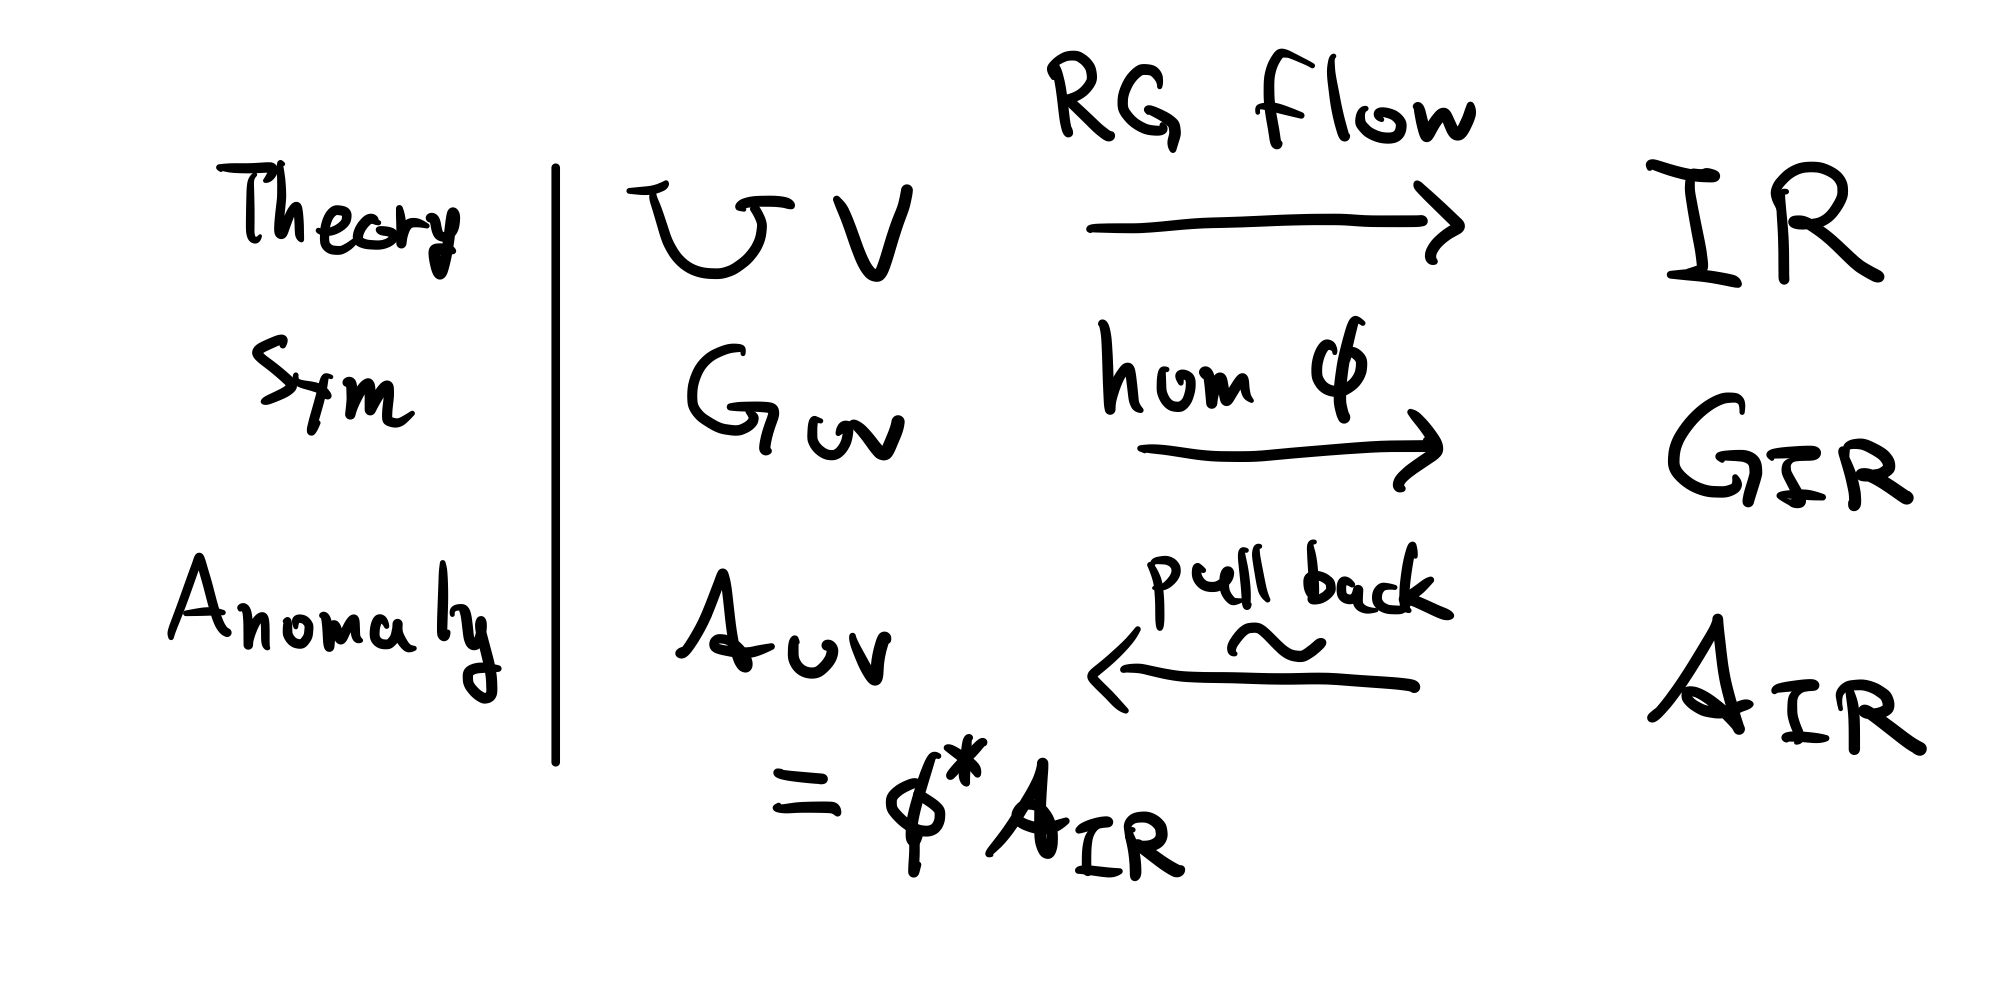
\includegraphics[width=0.5\linewidth]{figs/flow_symmetry} 

}

\caption{'t Hooft anomaly matching}\label{fig:flow}
\end{figure}

\hypertarget{quantum-anomaly-in-quantum-mechanics}{%
\section{Quantum Anomaly in Quantum Mechanics}\label{quantum-anomaly-in-quantum-mechanics}}

In this chapter we learn about quantum anomaly of a symmetry in quantum mechanics, without assuming any kind of locality.
Here, locality roughly means that we have a notion of ``observables localized in a subregion of the space (or spacetime).''
Both quantum field theory (QFT) and a quantum system on lattice are local in this sence, which greatly affect the possible behavior of a symmetry.
Here we will see what kind of ``topological'' phenomena are possible regarding symemtry when the locality is absent.
In such case, we often regard that all of the observables are associated to a single point consisting the entire ``space'', justifying call such a system ``0+1-dimensional.''

\hypertarget{basics-about-quantum-mechanics}{%
\subsection{Basics about quantum mechanics}\label{basics-about-quantum-mechanics}}

Let us recall the basics.
Given a quantum system, we have a Hilbert space \(\mathcal{H}\),
in which a state lives.
\(\ket{1}\)

\hypertarget{test}{%
\subsection{test}\label{test}}

test

\printbibliography

\end{document}
